\documentclass[12pt,a4paper]{article}
% 12pt:     Tamaño de fuente
% a4papper: Tamaño de papel
% article:  Formato artículo, está dividido por secciones y subsecciones. Otros formatos: report, letter, book, etc.

\usepackage[spanish, es-tabla]{babel}
% Configura en español los nombres de figuras, tablas, etc.
\usepackage[utf8]{inputenc}                 % Permite el uso directo de tildes y otros.
\usepackage{amsmath,amssymb}
% Añade símbolos matemáticos para las ecuaciones.
\usepackage{parskip}
% Elimina la sangría
\usepackage{geometry}
% Permite modificar los márgenes de la página a gusto.
\usepackage{multicol}
% Ordena el cuerpo del documento en 2 o más columnas.
\usepackage{graphicx}
% Para poner imágenes.
\usepackage{enumitem}
% Para modificar los tags de los enumerate.
\usepackage{array}
% Para ordenar texto y ecuaciones.
\usepackage{url}
% Permite usar url que redirigen a la página web.
\usepackage{hyperref}
% Permite que se puedan clickear las urls, citas y referencias.

\spanishdecimal{.} % punto decimal
\geometry{margin=2cm} % margenes de la hoja
\renewcommand{\baselinestretch}{1.3} % tamaño de las filas de las tablas

\newcommand{\uveci}{\hat{\imath}} % vector unitario i
\newcommand{\uvecj}{\hat{\jmath}} % vector unitario j
\newcommand{\uveck}{\hat{k}} % vector unitario k

\begin{document}

\begin{center}
{\Large\textbf{INFORME N°2}}

{\LARGE\textbf{Suma vectorial y equilibrio de fuerzas}}

\rule{\textwidth}{0.5pt}

\begin{tabular}{ll}
    \textbf{Estudiantes:} & Nombre Apellido \\
                          & Nombre Apellido \\
                          & Nombre Apellido \\
                          & Nombre Apellido \\[0.2cm]
    \textbf{Profesora:}   & Nombre Apellido \\
    \textbf{Ayudantes:}    & Nombre Apellido \\
                           & Nombre Apellido\\[0.2cm]
    \textbf{Fecha de entrega:} & DD de mes de AAAA
\end{tabular}

\vspace{0.4cm}
\rule{\textwidth}{0.5pt}

\end{center}

% ==========================================
% INCLUSIÓN DE LAS SECCIONES DEL INFORME
% ==========================================

\section{Procedimiento experimental}\subsection{Parte 1 - Mediciones experimentales y suma gráfica de vectores} \label{Procedimiento-Parte-1}Describan el procedimiento general utilizado para la realización de la medición de fuerzas y ángulos, la construcción de las configuraciones de equilibrio en la tabla de fuerzas y la representación gráfica de las fuerzas:\begin{enumerate}[label=\alph*)]
\item cómo definieron el sistema de referencia para los ángulos;
\item cómo realizaron las mediciones directas de las masas y los ángulos, con la resolución de los instrumentos;
\item cómo realizaron las mediciones indirectas de las fuerzas $\vec{F}_1$;
\item el procedimiento paso a paso para ajustar las tres configuraciones de equilibrio usando las cuerdas, poleas, resorte y dinamómetros;
\item cómo construyeron la representación gráfica vectorial de los sistemas y el método del polígono (ya sea en papel milimetrado, software de edición o Python).
\end{enumerate}\subsection{Parte 2 - Tratamiento analítico y propagación de error} \label{Procedimiento-Parte-2}Describan el desarrollo analítico utilizado para el cálculo de las componentes cartesianas de las fuerzas y sus respectivas incertidumbres absolutas.Para las componentes $x$:
\begin{align*}
F_x &= F \cos\theta \
\Delta F_x &= \sqrt{\left(\frac{\partial F_x}{\partial F}\delta F\right)^2 + \left(\frac{\partial F_x}{\partial \theta}\delta \theta_{\text{rad}}\right)^2} = \sqrt{\left(\cos\theta , \Delta F\right)^2 + \left(-F\sin\theta , \left(\Delta \theta \frac{\pi}{180^\circ}\right)\right)^2}
\end{align*}Para las componentes $y$:
\begin{align*}
F_y &= F \sin\theta \
\Delta F_y &= \sqrt{\left(\frac{\partial F_y}{\partial F}\delta F\right)^2 + \left(\frac{\partial F_y}{\partial \theta}\delta \theta_{\text{rad}}\right)^2} = \sqrt{\left(\sin\theta , \Delta F\right)^2 + \left(F\cos\theta , \left(\Delta \theta \frac{\pi}{180^\circ}\right)\right)^2}
\end{align*}Asimismo, detallen la forma analítica de calcular las componentes del vector resultante $\vec{R}_{\text{exp}}$ y sus incertidumbres $\Delta R_x$ y $\Delta R_y$:
\begin{align*}
R_x &= F_{1x} + F_{2x} + F_{3x}, \qquad \Delta R_x = \sqrt{\Delta F_{1x}^2 + \Delta F_{2x}^2 + \Delta F_{3x}^2} \
R_y &= F_{1y} + F_{2y} + F_{3y}, \qquad \Delta R_y = \sqrt{\Delta F_{1y}^2 + \Delta F_{2y}^2 + \Delta F_{3y}^2}
\end{align*}\subsection{Parte 3 - Comparación con la predicción teórica y análisis gráfico} \label{Procedimiento-Parte-3}Describan cómo construyeron el gráfico de puntos con barras de error para las componentes de los vectores resultantes y cómo lo interpretaron:\begin{enumerate}[label=\alph*)]
\item cómo definieron las variables de los ejes y sus escalas;
\item cómo incorporaron las barras de error en el gráfico;
\item cómo trazaron la línea de referencia teórica ($y = 0\,\mathrm{N}$) y qué significa;
\item el criterio utilizado para determinar si el resultado es compatible con el equilibrio.
\end{enumerate}

\newpage

\section{Configuración de Equilibrio 1}Describan brevemente la primera configuración de equilibrio, considerando la cantidad de masas suspendidas, la disposición de los dinamómetros y los ángulos seleccionados.\begin{table}[h!]
\centering
\begin{tabular}{|c|c|c|}
\hline
\textbf{Fuerza} & \textbf{Módulo ($F \pm \delta F$)} & \textbf{Ángulo ($\theta \pm \delta \theta$)} \\ \hline
$F_1$ & & \\ \hline
$F_2$ & & \\ \hline
$F_3$ & & \\ \hline
\end{tabular}
\caption{Medición directa e indirecta de módulos y ángulos para la Configuración 1.}
\label{tab:config1-mediciones}
\end{table}Los datos recolectados de esta configuración fueron registrados en la Tabla \ref{tab:config1-mediciones}. La representación gráfica de los vectores de esta configuración se puede ver en la Fig. \ref{fig:config1-vectores}.\begin{figure}[h!]
\centering
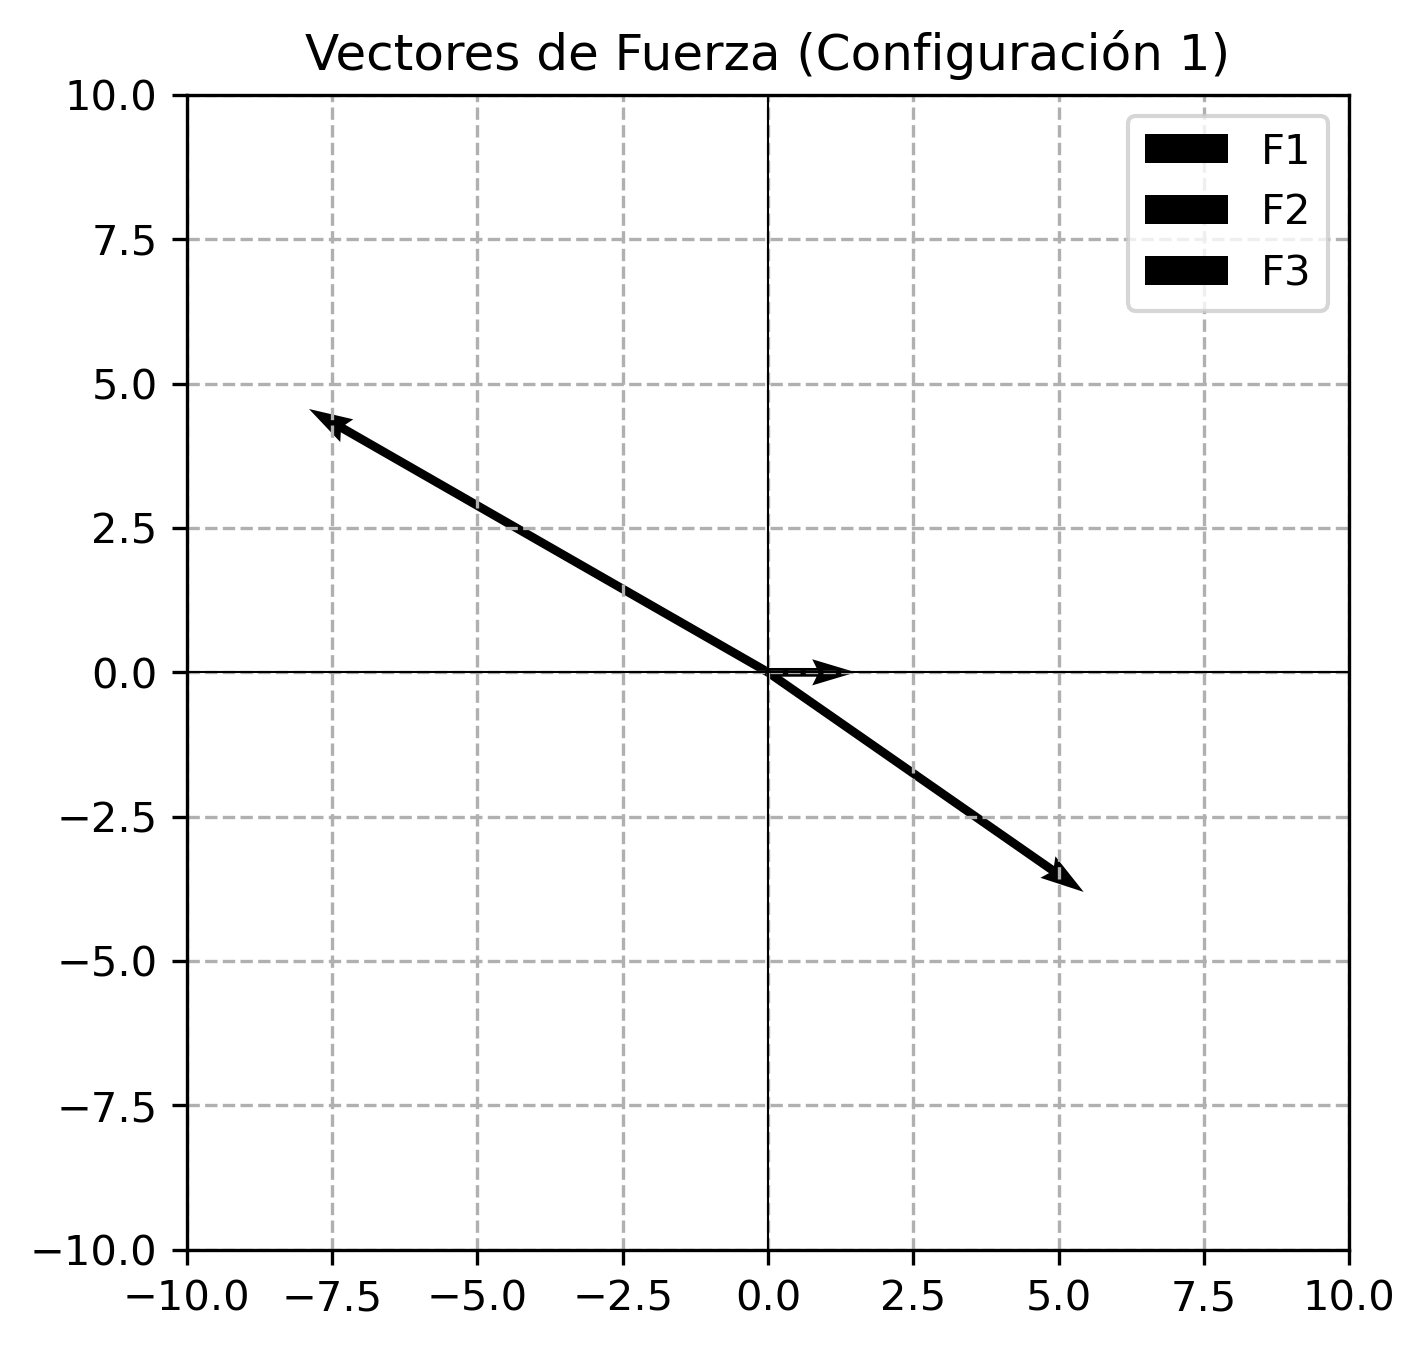
\includegraphics[width=0.4\textwidth]{config1-vectores.png}
\caption{Representación en el sistema de referencia de los vectores $\vec{F}_1$, $\vec{F}_2$ y $\vec{F}_3$ (Configuración 1).}
\label{fig:config1-vectores}
\end{figure}El módulo de $\vec{F}_1$ corresponde al peso de la masa, calculado como $F_1 = mg$. Para obtener $\delta F_1$, se realizó propagación de error.
\begin{equation*}
F_1 = mg = \dots
\end{equation*}
\begin{equation*}
\delta F_1 = \sqrt{\left(\frac{\partial F}{\partial m} \Delta m \right)^2 + \left(\frac{\partial F}{\partial g} \Delta g \right)^2} = \dots
\end{equation*}\subsection{Suma gráfica}La suma gráfica de los vectores se puede ver en la Fig. \ref{fig:config1-poligono}.\begin{figure}[h!]
\centering
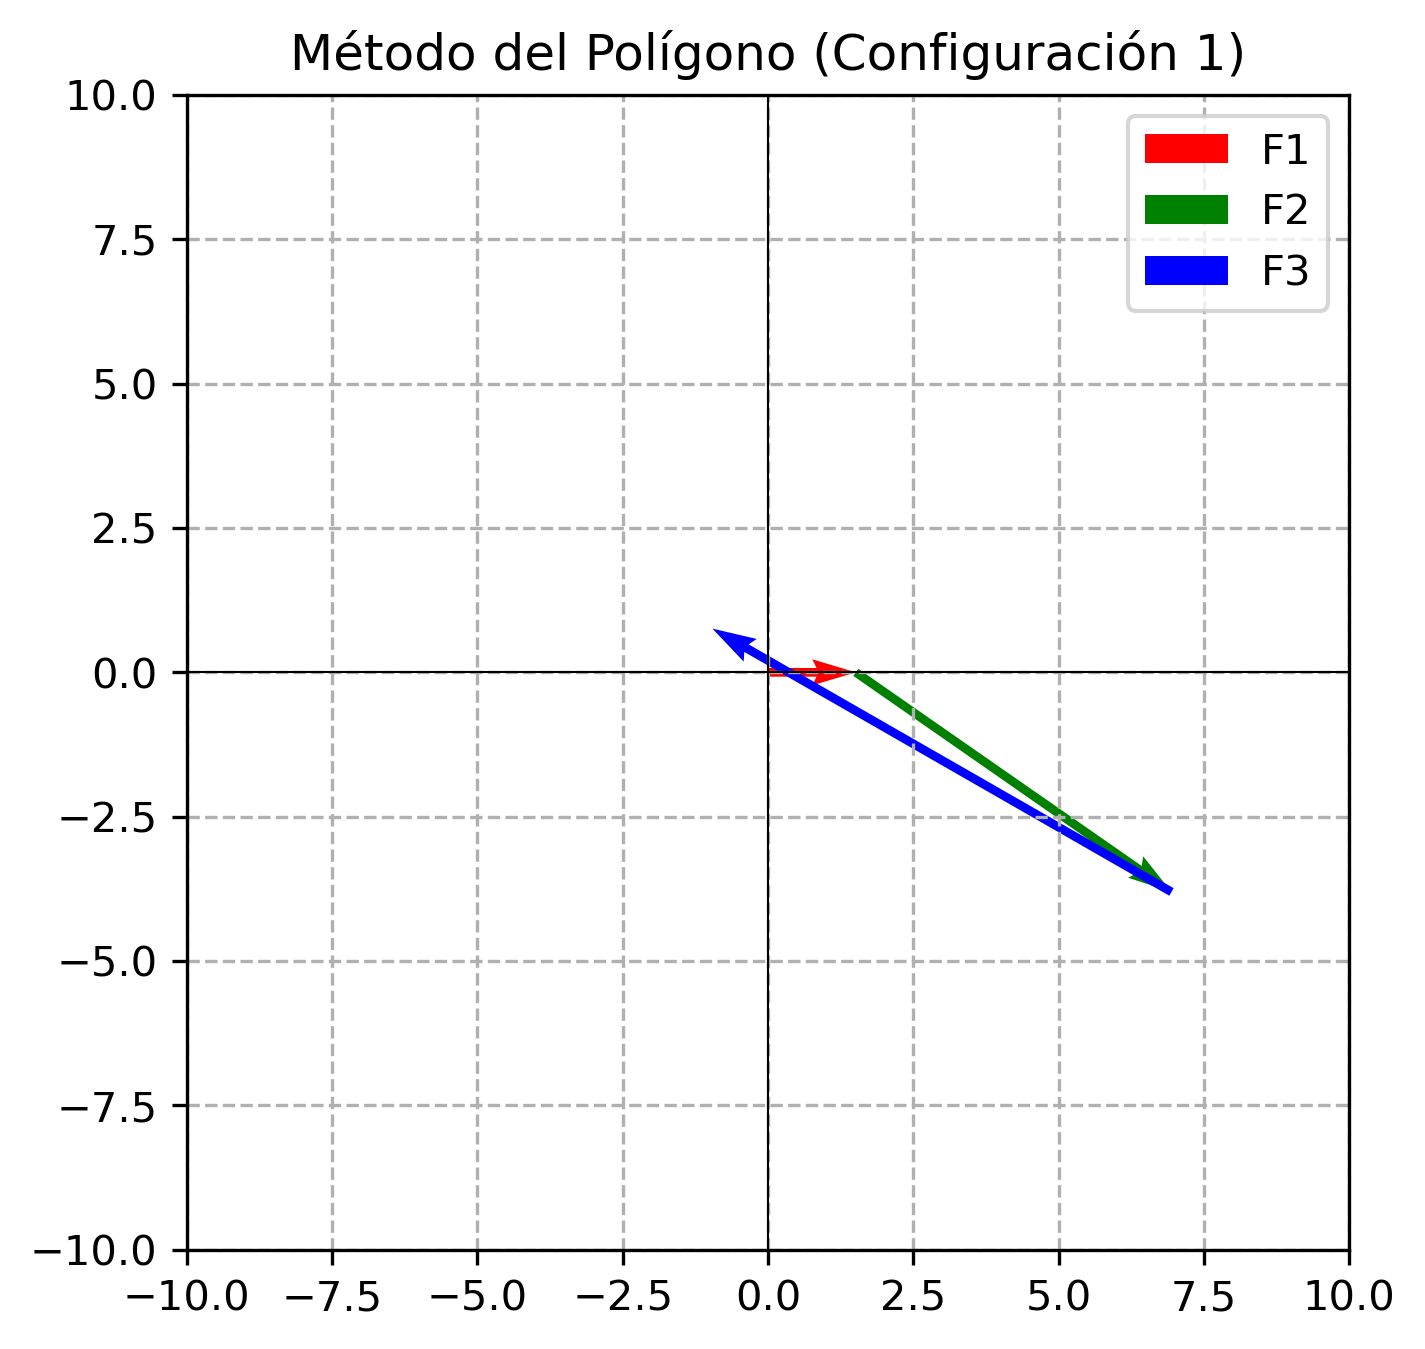
\includegraphics[width=0.4\textwidth]{config1-poligono.png}
\caption{Suma gráfica mediante el método del polígono para la Configuración 1.}
\label{fig:config1-poligono}
\end{figure}Comenten cualitativamente si el polígono se cierra correctamente o si existe alguna discrepancia gráfica visible.\subsection{Suma analítica}Los vectores de la Configuración 1 separados en sus componentes están registrados en la Tabla \ref{tab:config1-componentes}.\begin{table}[h!]
\centering
\begin{tabular}{|c|c|c|}
\hline
\textbf{Fuerza} & $F_x \pm \Delta F_x\,\mathrm{(N)}$ & $F_y \pm \Delta F_y\,\mathrm{(N)}$ \\ \hline
$F_1$ & & \\ \hline
$F_2$ & & \\ \hline
$F_3$ & & \\ \hline
\end{tabular}
\caption{Componentes cartesianas e incertidumbres absolutas para la Configuración 1.}
\label{tab:config1-componentes}
\end{table}Sumando estas componentes, el vector resultante es:\begin{equation*}
\vec{R}_{\mathrm{exp, 1}} = (R_x \pm \Delta R_x),\uveci + (R_y \pm \Delta R_y),\uvecj = (\dots \pm \dots),\uveci + (\dots \pm \dots),\uvecj,\mathrm{N}
\end{equation*}\subsection{Comparación de los resultados}La Fig. \ref{fig:grafico-error-1} muestra la comparación gráfica entre la predicción teórica y el resultado experimental.\begin{figure}[h!]
\centering
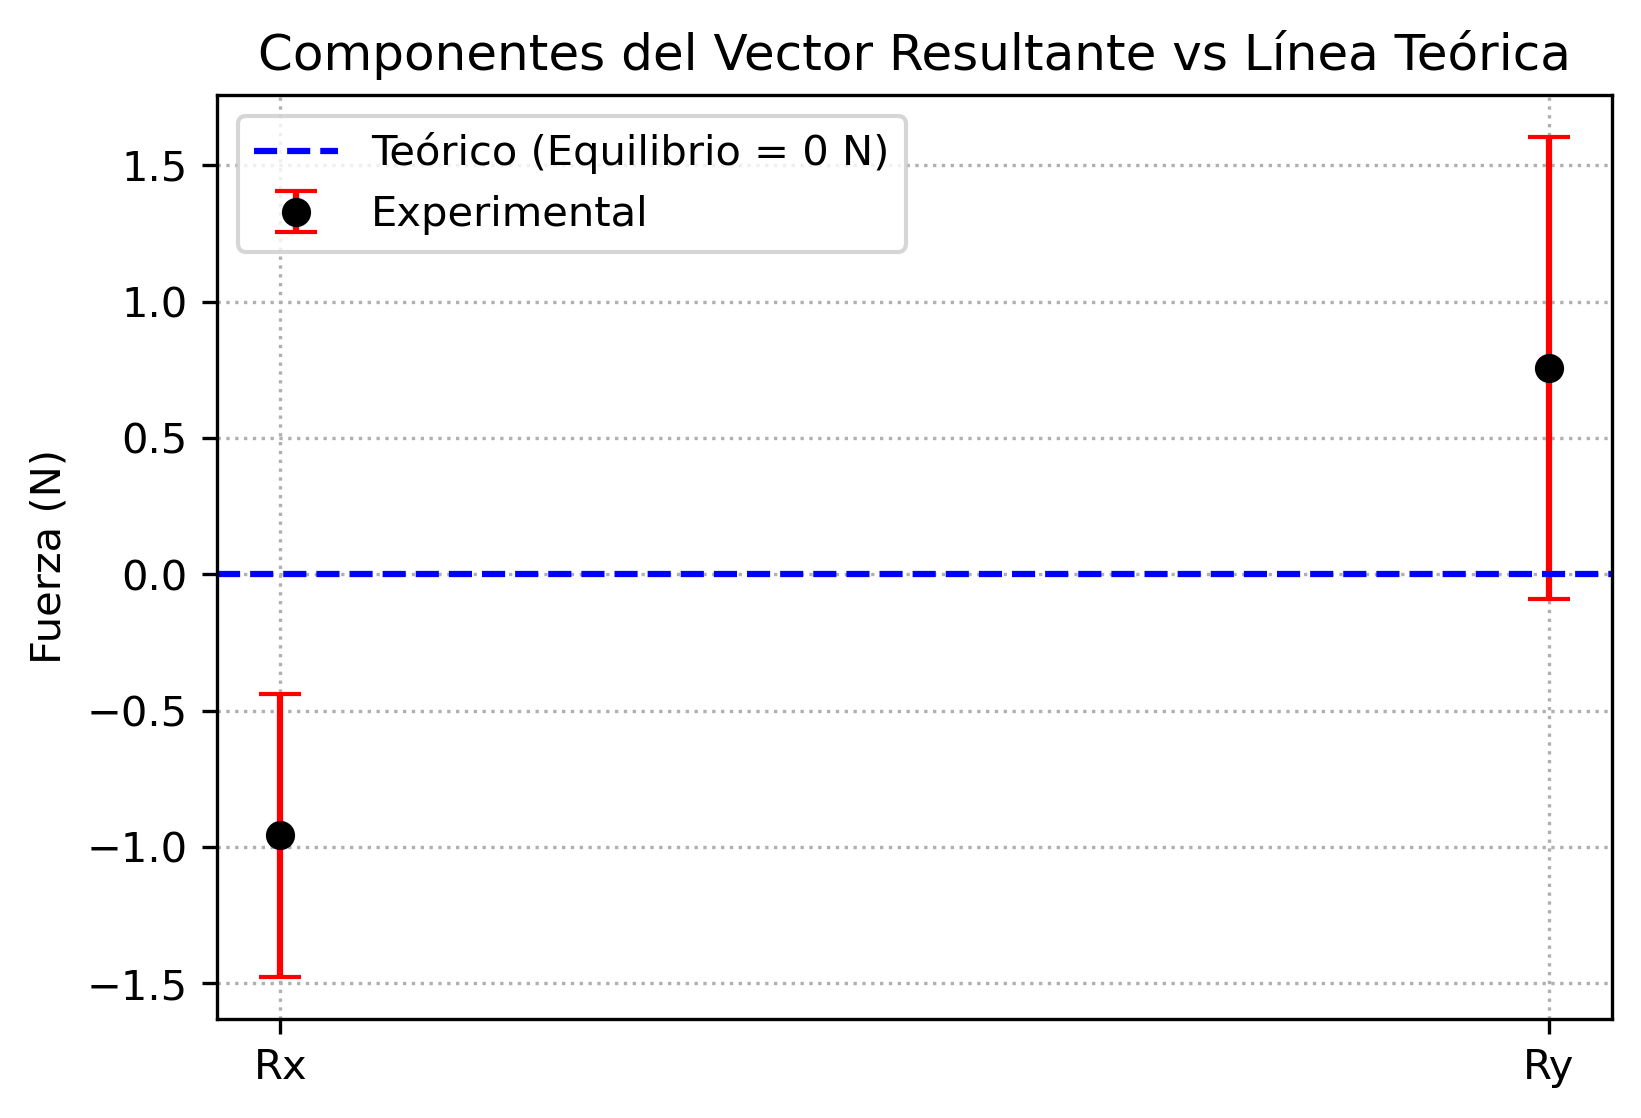
\includegraphics[width=0.4\textwidth]{grafico-error-config1.png}
\caption{Gráficos de las componentes de la fuerza resultante $R_x$ y $R_y$ con barras de error en relación a la referencia teórica $y=0\,\mathrm{N}$ para la Configuración 1.}
\label{fig:grafico-error-1}
\end{figure}Describan y analicen el gráfico obtenido. Indiquen si las barras de error de las componentes $R_x$ y $R_y$ cruzan la línea de referencia $y = 0\,\mathrm{N}$ y qué concluyen a partir de dicho cruce sobre la compatibilidad experimental con la condición de equilibrio traslacional.

\newpage

\input{3_configuracion2.tex}
\newpage

\section{Configuración de Equilibrio 3}Describan la tercera configuración de equilibrio utilizada, considerando la cantidad de masas suspendidas, la disposición de los dinamómetros y los ángulos seleccionados.\begin{table}[h!]
\centering
\begin{tabular}{|c|c|c|}
\hline
\textbf{Fuerza} & \textbf{Módulo ($F \pm \delta F$)} & \textbf{Ángulo ($\theta \pm \delta \theta$)} \\ \hline
$F_1$ & & \\ \hline
$F_2$ & & \\ \hline
$F_3$ & & \\ \hline
\end{tabular}
\caption{Medición directa e indirecta de módulos y ángulos para la Configuración 3.}
\label{tab:config3-mediciones}
\end{table}Los datos recolectados de esta configuración fueron registrados en la Tabla \ref{tab:config3-mediciones}. El módulo de $\vec{F}_1$ corresponde al peso de la masa, calculado como $F_1 = mg$. Para obtener $\delta F_1$, se realizó propagación de error.
\begin{equation*}
F_1 = mg = \dots
\end{equation*}
\begin{equation*}
\delta F_1 = \sqrt{\left(\frac{\partial F}{\partial m} \Delta m \right)^2 + \left(\frac{\partial F}{\partial g} \Delta g \right)^2} = \dots
\end{equation*}La representación gráfica de los vectores de esta configuración se puede ver en la Fig. \ref{fig:config3-vectores}.\begin{figure}[h!]
\centering
\includegraphics[width=0.4\textwidth]{config3-vectores.png}
\caption{Representación en el sistema de referencia de los vectores $\vec{F}_1$, $\vec{F}_2$ y $\vec{F}_3$ (Configuración 3).}
\label{fig:config3-vectores}
\end{figure}\subsection{Suma gráfica de los vectores de la Configuración 3}La suma gráfica de los vectores se puede ver en la Fig. \ref{fig:config3-poligono}.\begin{figure}[h!]
\centering
\includegraphics[width=0.4\textwidth]{config3-poligono.png}
\caption{Suma gráfica mediante el método del polígono para la Configuración 3.}
\label{fig:config3-poligono}
\end{figure}Comenten cualitativamente si el polígono se cierra correctamente o si existe alguna discrepancia gráfica visible.\subsection{Suma analítica de los vectores de la Configuración 3}Los vectores de la Configuración 3 separados en sus componentes están registrados en la Tabla \ref{tab:config3-componentes}.\begin{table}[h!]
\centering
\begin{tabular}{|c|c|c|}
\hline
\textbf{Fuerza} & $F_x \pm \Delta F_x\,\mathrm{(N)}$ & $F_y \pm \Delta F_y\,\mathrm{(N)}$ \\ \hline
$F_1$ & & \\ \hline
$F_2$ & & \\ \hline
$F_3$ & & \\ \hline
\end{tabular}
\caption{Componentes cartesianas e incertidumbres absolutas para la Configuración 3.}
\label{tab:config3-componentes}
\end{table}Sumando estas componentes, el vector resultante es:\begin{equation*}
\vec{R}_{\mathrm{exp, 3}} = (R_x \pm \Delta R_x),\uveci + (R_y \pm \Delta R_y),\uvecj = (\dots \pm \dots),\uveci + (\dots \pm \dots),\uvecj,\mathrm{N}
\end{equation*}\subsection{Comparación de los resultados}La Fig. \ref{fig:grafico-error-3} muestra la comparación gráfica entre la predicción teórica y el resultado experimental.\begin{figure}[h!]
\centering
\includegraphics[width=0.4\textwidth]{grafico-error-config3.png}
\caption{Gráficos de las componentes de la fuerza resultante $R_x$ y $R_y$ con barras de error en relación a la referencia teórica $y=0\,\mathrm{N}$ para la Configuración 3.}
\label{fig:grafico-error-3}
\end{figure}Describan y analicen el gráfico obtenido. Indiquen si las barras de error de las componentes $R_x$ y $R_y$ cruzan la línea de referencia $y = 0\,\mathrm{N}$ y qué concluyen a partir de dicho cruce sobre la compatibilidad experimental con la condición de equilibrio traslacional.

\newpage

\section{Análisis y conclusiones}

En esta sección, resuman brevemente lo realizado en el laboratorio. Indiquen qué se hizo y cuál fue el propósito de cada actividad, haciendo referencia a las secciones, tablas y ecuaciones correspondientes cuando sea necesario. No es necesario volver a enunciar todos los datos o repetir los procedimientos detallados anteriormente. El resumen puede realizarse en un solo párrafo o en tres párrafos distintos, uno para cada parte.

Luego del resumen de las actividades, respondan las preguntas de análisis planteadas en las tres partes de la guía. Pueden presentar todas las respuestas en un solo texto o separarlas en tres párrafos, uno para cada actividad. En cada respuesta, no se limiten a indicar un resultado: expliquen el razonamiento que utilizaron para llegar a él y relacionen sus conclusiones con los datos, cálculos y gráficos obtenidos durante el trabajo. Las respuestas a las preguntas de análisis deben estar integradas en el texto, conectando ideas mediante conectores lógicos. Eviten presentar las respuestas de manera aislada, como en formato pregunta-respuesta.

Finalmente, incluyan las principales conclusiones a las que llegaron como grupo. Estas deben sintetizar los aprendizajes obtenidos a partir de las actividades realizadas y destacar los aspectos que consideren más relevantes respecto de la medición de magnitudes físicas, el tratamiento de datos y su representación gráfica. Cuando corresponda, indiquen también las principales limitaciones o fuentes de incertidumbre que hayan identificado durante el trabajo.

Las conclusiones deben basarse en los resultados obtenidos por el grupo. \textbf{No incluyan citas bibliográficas en esta sección}.

\textbf{\underline{Extensión máxima del informe:} indefinida}.


% ==========================================

\begin{thebibliography}{99}

\bibitem{libro} Nombre del autor. \textit{Título del libro}. Año.

\bibitem{apunte} Nombre del profesor. \textit{Nombre del curso}. Semestre y año en el que fue entregado el apunte.

\bibitem{web} TikTok de @usuario. Disponible en: \url{https://www.tiktok.com/}.

\end{thebibliography}

\end{document}

